\documentclass{standalone}

\usepackage{tikz}

\begin{document}
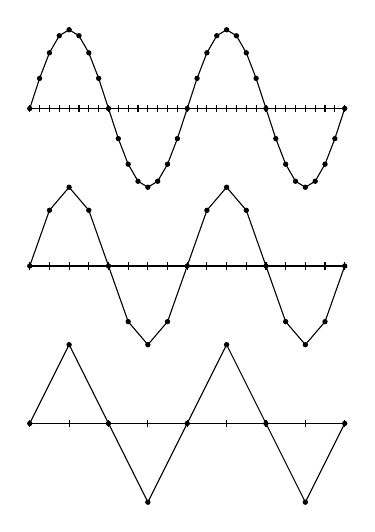
\begin{tikzpicture}[mark size=.75pt]
	\def\tick{.05}
	\draw (0,-\tick) grid[step=.125] (4,\tick); 
	\draw[domain=0:4, samples=33] plot[mark=*] (\x, {sin(\x*180)}); 

	\begin{scope}[yshift=-2cm]
		\draw (0,-\tick) grid[step=.25] (4,\tick); 
		\draw[domain=0:4, samples=17] plot[mark=*] (\x, {sin(\x*180)}); 
	\end{scope}
	\begin{scope}[yshift=-4cm]
		\draw (0,-\tick) grid[step=.5] (4,\tick); 
		\draw[domain=0:4, samples=9] plot[mark=*] (\x, {sin(\x*180)}); 
	\end{scope}
\end{tikzpicture}
\end{document}